\section{Week-end entre amies (4 points)}

Trois amies vivent dans trois villes différentes. Elles souhaitent passer un week-end ensemble. Elles veulent parcourir la même distance <<à vol d'oiseau>>. Elles habitent à Lille, Strassbours et Bayonne.

\begin{center}
	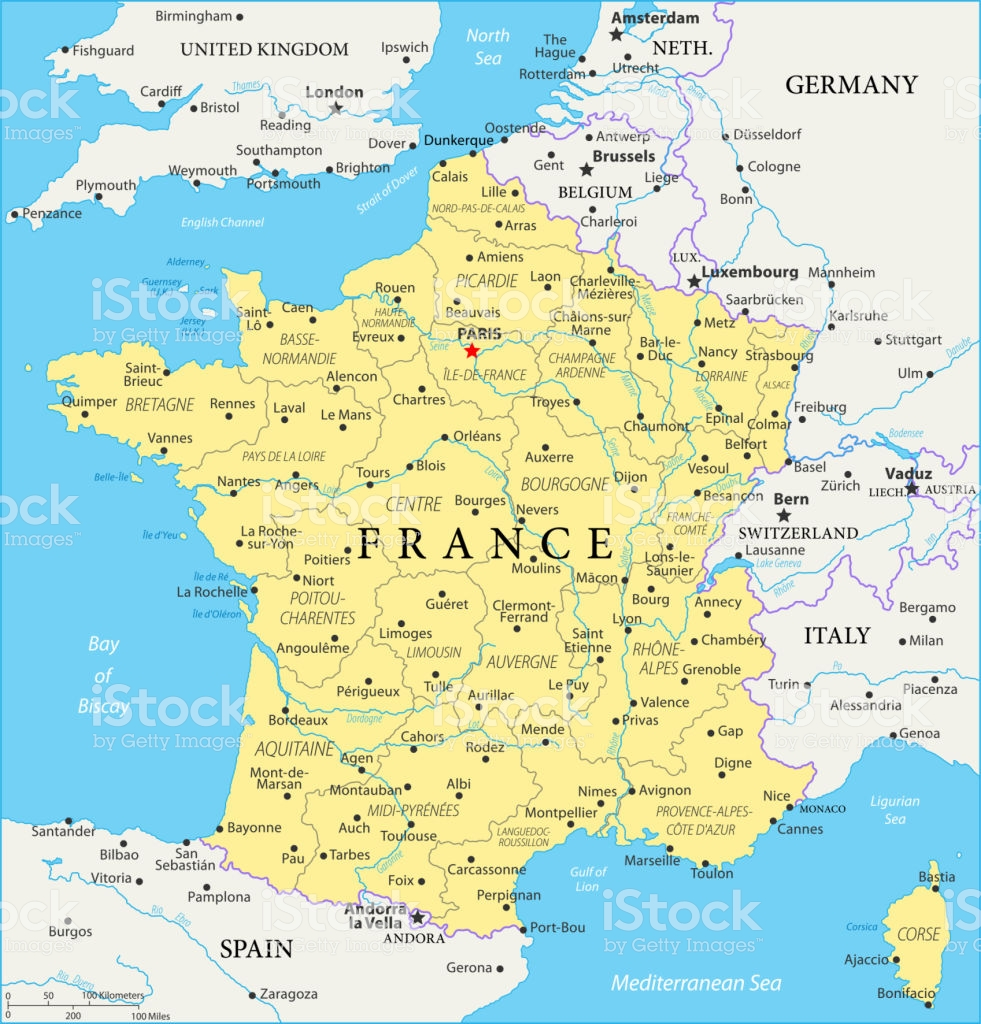
\includegraphics[scale=1.55]{img/france}
\end{center}

\begin{questions}
	\question[4] Trouver \textbf{\underline{sur cette carte}} l'endroit idéal pour leur week-end. Expliquer la démarche, laisser apparents tous les traits de construction et coder la figure.
\end{questions}

